\chapter{Design}
\section{Actors}
The main actors of the application are: 
\begin{itemize}
	\item \emph{Non-Logged User (Guest User)} : anonymous users that access the application. They can either sign up or log in.
	\item \emph{User} : end-user of the application.
	\item \emph{Company Manager} : it's a special kind of \emph{user}, who is granted more benefits. Company Managers identify Game Developers/Publishers that, as such, are able to view and run analytics over their own products. 
	\item \emph{Administrator} : \emph{users} that can run and view analytics that concern the whole database. They are the ones who manage the application: they are able to delete any type of content, update information about Games or Users and to ban them at the occurrence. 
\end{itemize}
\section{Requirements}
\subsection{Functional Requirements}
What follows is a list of the functional requirements.
\subsubsection{Guest User}
\begin{itemize}
	\item sign up
        \item log in
\end{itemize}
\subsubsection{All Users}
\begin{itemize}
	\item view other users' profiles
	\item view companies' profiles
	\item view information about videogames
\end{itemize}
\subsubsection{All Users except Guest Users}
\begin{itemize}
        \item view recommended games
	\item view recommended users
        \item follow/unfollow users
        \item "like" a review
	\item view and edit their profile info
        \item review a videogame
	\item comment on another user's review
\end{itemize}
\subsubsection{Company Manager Exclusive}
Note: all of the following apply only to games published or developed by the company the \emph{company manager} represents 
\begin{itemize}
	\item add a videogame to the database 
	\item modify info about a game 
	\item delete a videogame from the database 
	\item view the score distribution for the company's videogames
	\item view the top games by average score
	\item view the best game of the company (by average score)
\end{itemize}
\subsubsection{Administrator Exclusive}
\begin{itemize}
	\item delete ("ban") a user from the database
	\item delete a review from the database
	\item delete a comment from the database
	\item delete a videogame from the database 
	\item view the top users by number of likes received on their reviews
	\item view the top users by number of reviews published
	\item view the most active user (by number of reviews posted in the last 6 month)
	\item view the user with most likes received
	\item view the global distribution of the review score
\end{itemize}
\subsection{Non-Functional Requirements}
The following is a list of all non-functional requirements.
\begin{itemize}
	\item \emph{Usability}: the application must have a user-friendly interface and have low response times
	\item \emph{Availability}: the service provided by the application must be always available to all users
	\item \emph{Reliability}: the application must be stable during its use and it must return reproducible results
	\item \emph{Flexibility}: company managers should be able to add any attribute to a game they want to publish, and the application should account for this
	\item \emph{Portability}: the application must be executable in different operating systems without changes in its behaviour
	\item \emph{Privacy}: every user's information should be handled securely
	\item \emph{Maintainability}: the code should be modular and easy to read.
\end{itemize}
\section{Use Case Diagram}
We can look at the use case diagram of the application in Figure \ref{fig:usecase}
\begin{figure}[hbt!]
	\centering
	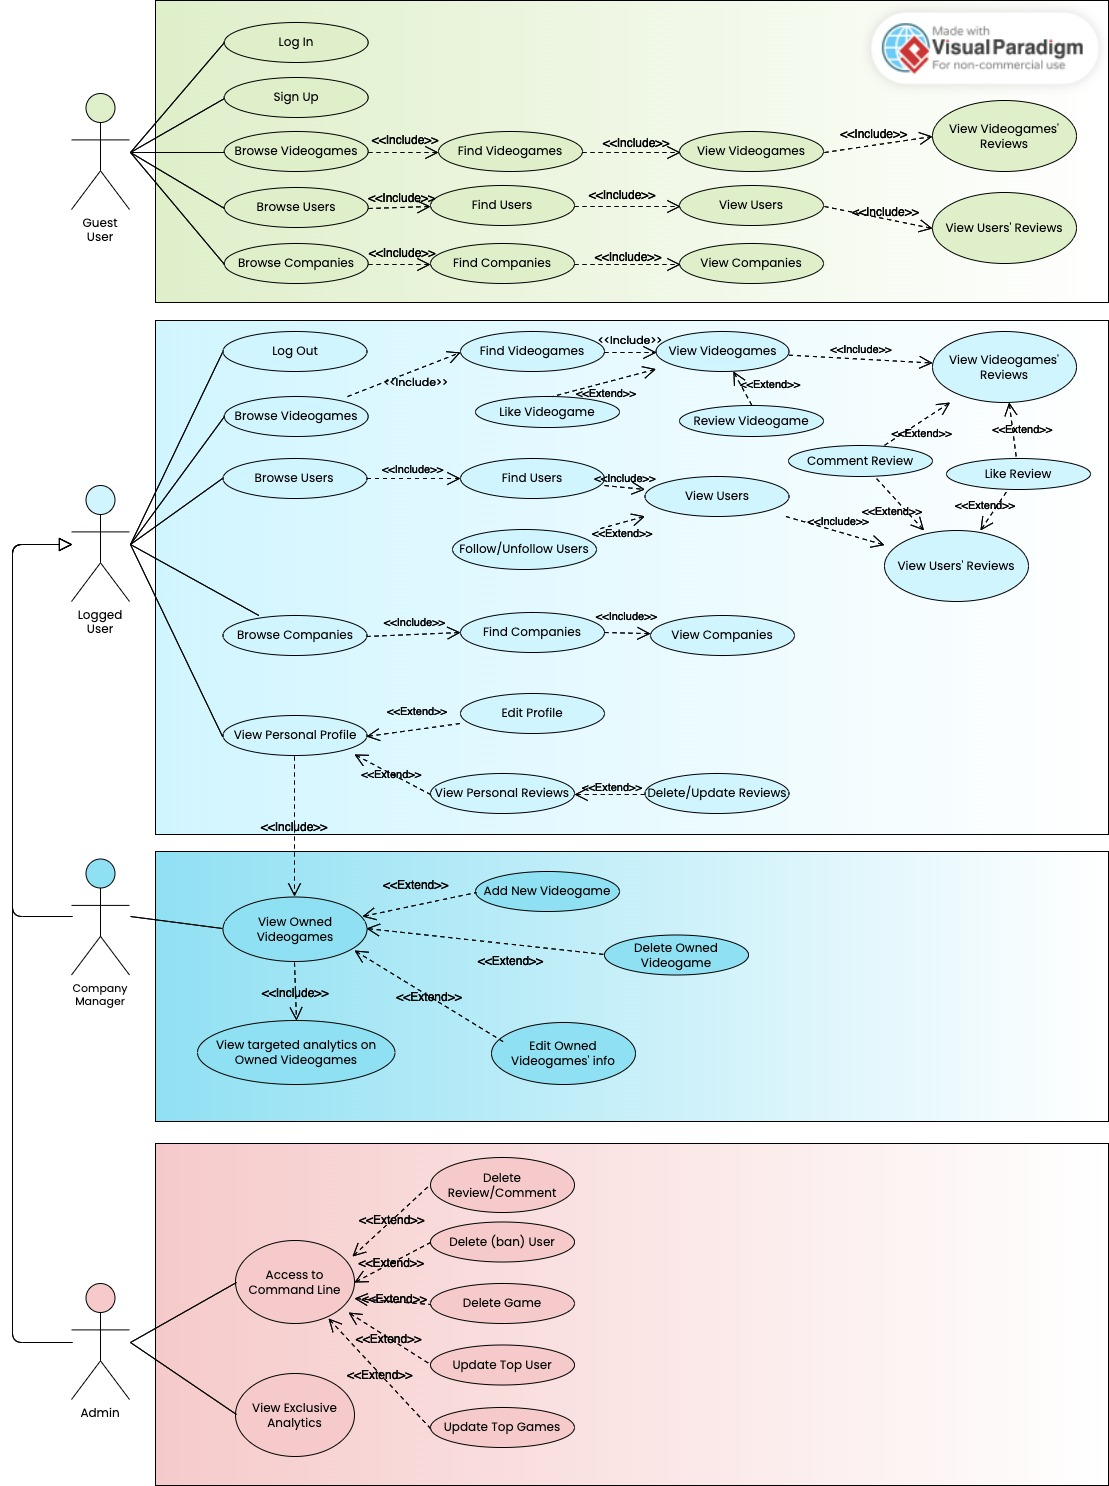
\includegraphics[width=1\textwidth]{chapter3/img/usecase.jpg}
	\caption{Actors and main supported functionalities}
	\label{fig:usecase}
\end{figure}
\emph{Guest users} are able to look at all the content available on the platform, but they can not either review videgames, comment reviews or like them, all actions that only registered users (\emph{Simple Users} that are logged) can perform. 
Users registered as \emph{Company Managers}, that are associated to some specific \emph{Company} that either developed or published \emph{Videogames} available on the platform, are given the possibility to perform some specific actions in order to assess the consumers' sentiment regarding their products. Moreover they are able to edit the pages related to their own \emph{Videogames}. 
\emph{Admin Users} are the ones that handle the content over the whole platform. 
Both \emph{Company Managers} and \emph{Administrators} can still perform all actions linked to a \emph{Simple User}. 
\section{UML Class Diagram}
\begin{figure}[hbt!]
	\centering
	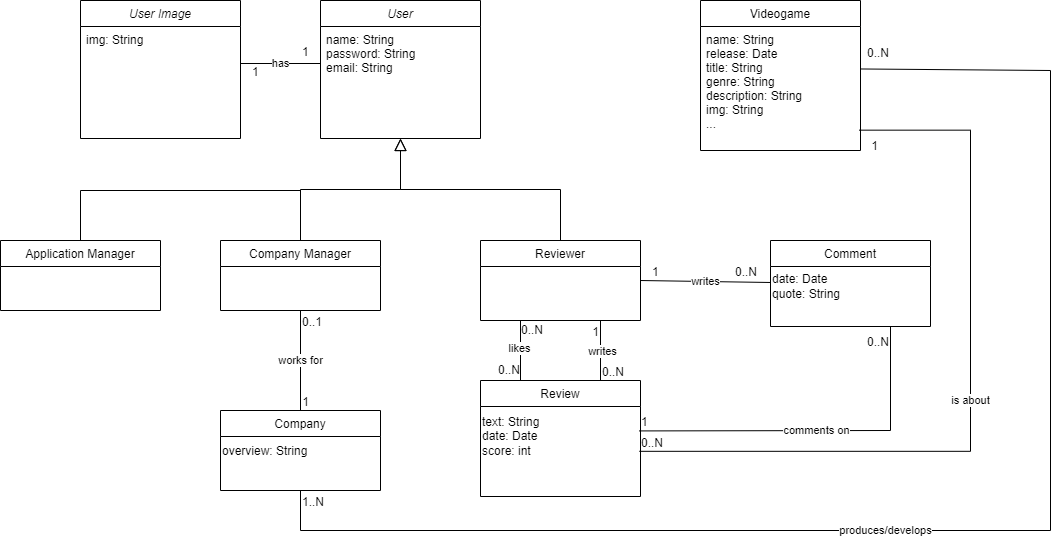
\includegraphics[width=1\textwidth]{chapter3/img/uml.png}
	\caption{UML Class Diagram}
	\label{fig:uml}
\end{figure}
The UML class diagram is reported in Figure \ref{fig:uml}
\subsection{Relationships between classes}
\begin{itemize}
    \item A \emph{User} can be either be a \emph{Simple User}, a \emph{Company Manager} or an \emph{Administrator}. 
    \item a \emph{User}, whatever its specific role, can be associated with zero or more \emph{Reviews} they have written
    \item Each \emph{Review} has a specific author (it is written by one \emph{User} alone)
    \item a \emph{User} can like zero or more \emph{Reviews}
    \item Each \emph{Review} may have been liked by zero or more \emph{Users}
    \item a \emph{User} may have written zero or more \emph{Comments} attached to some \emph{Review} (either written by themselves or by other \emph{Users})
    \item Each \emph{Comment} has a specific author (\emph{User})
    \item Each \emph{User} has a \emph{User Image} linked to their personal profile (a default Image gets associated to each user, that then has the possibility to change it by editing his personal profile)
    \item Each \emph{User Image} is linked to a specific \emph{User}
    \item Each \emph{Comment} is related to one specific \emph{Review}
    \item Each \emph{Review} may have zero or more \emph{Comments}
    \item Each \emph{Review} is associated to a specific \emph{Videogame} 
    \item Each \emph{Videogame} may have zero or more \emph{Reviews} that talk about it
    \item Every \emph{Videogame} is linked to one or more \emph{Companies}, that either developed or published it
    \item Each \emph{Company} registered on the platform is associated to zero or more \emph{Videogames} 
    \item Every \emph{Company Manager} is linked to the \emph{Company} they work for 
    \item Each \emph{Company} may or may not have one \emph{Company Manager} registered as a user (with privileges discussed later on) over the platform 
\end{itemize}
\subsection{Design of the classes}
Here we offer a brief description of some of the entities' attributes
\subsubsection{User - Simple User, Company Manager, Admin}
\begin{itemize}
    \item \texttt{name} : a string that contains the username associated to a specific user. It is unique for each user stored inside the database
    \item \texttt{password} : string that contains the hash of the password the user has to enter in order to log in 
    \item \texttt{email} : a string that contains the email offered during the \emph{sign up} procedure to create an account 
\end{itemize}
\subsubsection{Review}
\begin{itemize}
    \item \texttt{quote} : a string that contains the text of the review 
    \item \texttt{date} : timestamp that keeps track of the day the review has been posted 
    \item \texttt{score} : an integer that represents the review score - ranging from 0 to 10 - that is linked to the review and is used to make analytics
\end{itemize}
\subsubsection{Comment}
\begin{itemize}
    \item \texttt{date} : timestamp that keeps track of the day the comment has been posted 
    \item \texttt{quote} : a string that contains the content of the comment 
\end{itemize}
\subsubsection{Videogame}
\begin{itemize}
    \item \texttt{name} : a string that contains name of the videogame 
    \item \texttt{release} : date on which the videogame was released
    \item \texttt{genre} : a string that contains the genre to which the game belongs to (i.g. Action, Platform Games, Adventure, Puzzle etc.)
    \item \texttt{description} : a string that contains a brief description of the videogame
    \item \texttt{img} : a string that contains the URL of the image of the videogame's cover
\end{itemize}
We listed the more common attributes, but we remember the number and the type of attributes may change from one videogame document to another 
\subsubsection{Company}
\begin{itemize}
    \item \texttt{overview} : a string that describes the profile of the company
\end{itemize}
\subsubsection{User Image}
\begin{itemize}
    \item \texttt{img} : a string that contains the URL of the image used as an icon to associate to a specific user 
\end{itemize}

